A modelagem estática da viga VL2 é apresentada abaixo:

\begin{figure}[H]
  \centering
  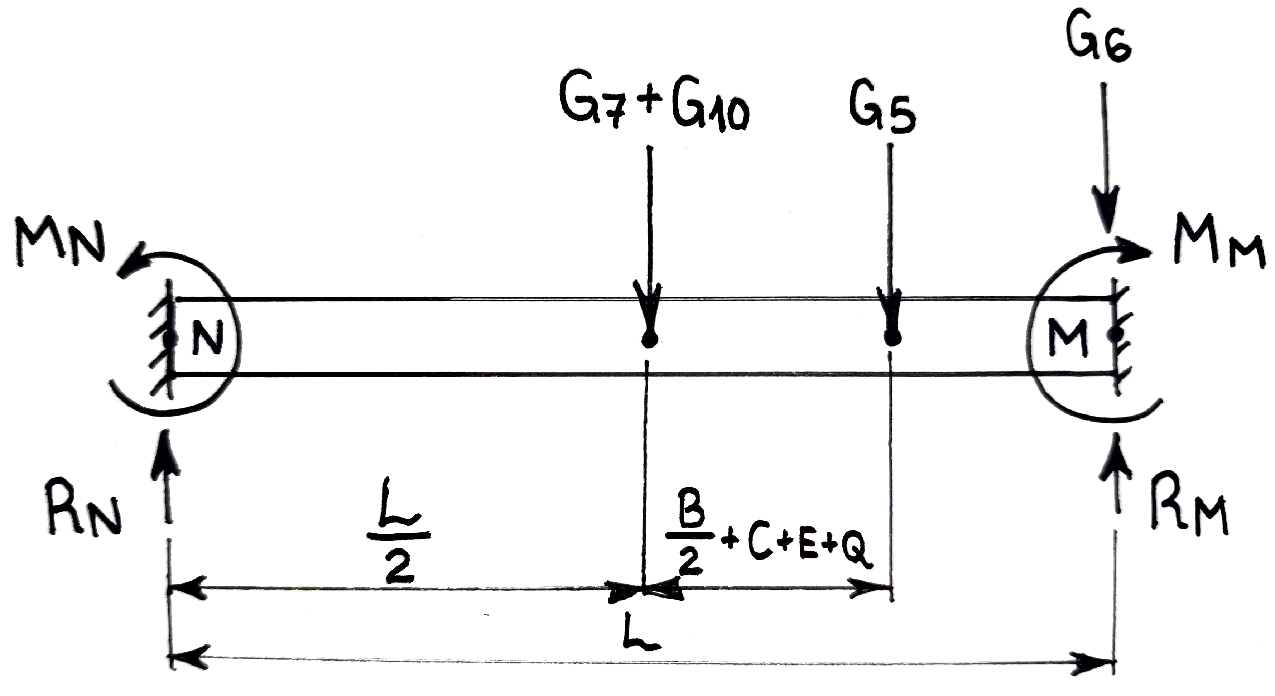
\includegraphics[width=0.8\textwidth]{content/sections/04_estrutura/sections/01_pre_dimensionamento_da_viga_vl2/figures/predim_vl2.pdf}
  \caption{Modelagem estática da viga VL2 (Autor)}
  \label{fig:predim_vl2}
\end{figure}

O comprimento do pórtico é obtido da seguinte forma:

\begin{equation}
  L = L_{\text{total}} + P - L_S
  \label{eq:comprimento_portico}
\end{equation}

Onde:

\begin{itemize}
  \item $L$: comprimento do pórtico em \si{\meter}.
  \item $L_{\text{total}}$: comprimento total do tambor em \si{\meter} \eqref{eq:comprimento_total_tambor}.
  \item $P$: centro do redutor até a ponta do eixo de saída em \si{\meter} (Tabela \ref{tab:dados_redutor_adotado}).
  \item $L_S$: comprimento do eixo de saída do redutor em \si{\meter} (Tabela \ref{tab:dados_redutor_adotado}).
\end{itemize}

\vspace{1em}

Substituindo os valores na equação \eqref{eq:comprimento_portico}:

\begin{align*}
  L & = \num{2.212} + \num{0.475} - \num{0.25} \\
  L & = \boxed{\SI{2.437}{\meter}}
\end{align*}

A distância do centro da viga até o peso do motor $G_5$ é obtida da seguinte forma:

\begin{equation}
  \text{distância} \ G_5 = \frac{B}{2} + C + E + Q
  \label{eq:dist_g5}
\end{equation}

Onde:

\begin{itemize}
  \item $B$: distância entre os furos da base do motor em \si{\meter} (Tabela \ref{tab:dados_motor_adotado}).
  \item $C$: furo dianteiro até a frente da carcaça do motor em \si{\meter} (Tabela \ref{tab:dados_motor_adotado}).
  \item $E$: comprimento do eixo do motor em \si{\meter} (Tabela \ref{tab:dados_motor_adotado}).
  \item $Q$: centro do redutor até a ponta do eixo de entrada em \si{\meter} (Tabela \ref{tab:dados_redutor_adotado}).
\end{itemize}

\vspace{1em}

Substituindo os valores na equação \eqref{eq:dist_g5}:

\begin{align*}
  \text{distância} \ G_5 & = \frac{\num{0.254}}{2} + \num{0.108} + \num{0.11} + \num{0.345} \\
  \text{distância} \ G_5 & = \boxed{\SI{0.69}{\meter}}
\end{align*}

O peso do freio de parada e da polia do freio é obtido da seguinte forma:

\begin{equation}
  G_6 = \left( M_{\text{freio}} + M_{\text{polia}} \right) \cdot g
  \label{eq:g6}
\end{equation}

Onde:

\begin{itemize}
  \item $G_6$: peso do freio de parada e da polia do freio em \si{\newton}.
  \item $M_{\text{freio}}$: massa do freio de parada em \si{\kilogram} (Tabela \ref{tab:dados_freio_adotado}).
  \item $M_{\text{polia}}$: massa da polia do freio em \si{\kilogram} (Tabela \ref{tab:dados_freio_adotado}).
  \item $g$: aceleração da gravidade em \si{\meter\per\second\squared}.
\end{itemize}

\vspace{1em}

Substituindo os valores na equação \eqref{eq:g6}:

\begin{align*}
  G_6 & = \left( \num{39} + \num{15} \right) \cdot 10 \\
  G_6 & = \boxed{\SI{540}{\newton}}
\end{align*}

Para o peso das polias de passagem e da polia de compensação, considerando \SI{80}{\kilo\gram} para cada polia, sendo 2 polias de passagem e 1 polia de compensação, o peso total, somado à tração do cabo, é obtido da seguinte forma:

\begin{equation}
  G_7 = 3 \cdot 80 \cdot g + 2 T
  \label{eq:g7}
\end{equation}

Onde:

\begin{itemize}
  \item $G_7$: peso das polias de passagem e da polia de compensação em \si{\newton}.
  \item $T$: tração do cabo em \si{\newton} \eqref{eq:forca_de_tracao_no_cabo}.
  \item $g$: aceleração da gravidade em \si{\meter\per\second\squared}.
\end{itemize}

\vspace{1em}

Substituindo os valores na equação \eqref{eq:g7}:

\begin{align*}
  G_7 & = 3 \cdot 80 \cdot 10 + 2 \cdot \num{25377.8} \\
  G_7 & = \boxed{\SI{53155.6}{\newton}}
\end{align*}

O peso do motor é obtido da seguinte forma:

\begin{equation}
  G_8 = M_{\text{motor}} \cdot g
  \label{eq:g8}
\end{equation}

Onde:

\begin{itemize}
  \item $G_8$: peso do motor em \si{\newton}.
  \item $M_{\text{motor}}$: massa do motor em \si{\kilogram} (Tabela \ref{tab:dados_motor_adotado}).
  \item $g$: aceleração da gravidade em \si{\meter\per\second\squared}.
\end{itemize}

\vspace{1em}

Substituindo os valores na equação \eqref{eq:g8}:

\begin{align*}
  G_8 & = \num{158} \cdot 10         \\
  G_8 & = \boxed{\SI{1580}{\newton}}
\end{align*}

Assim, é possível definir o diagrama de corpo livre (DCL) da viga VL2:

\begin{figure}[H]
  \centering
  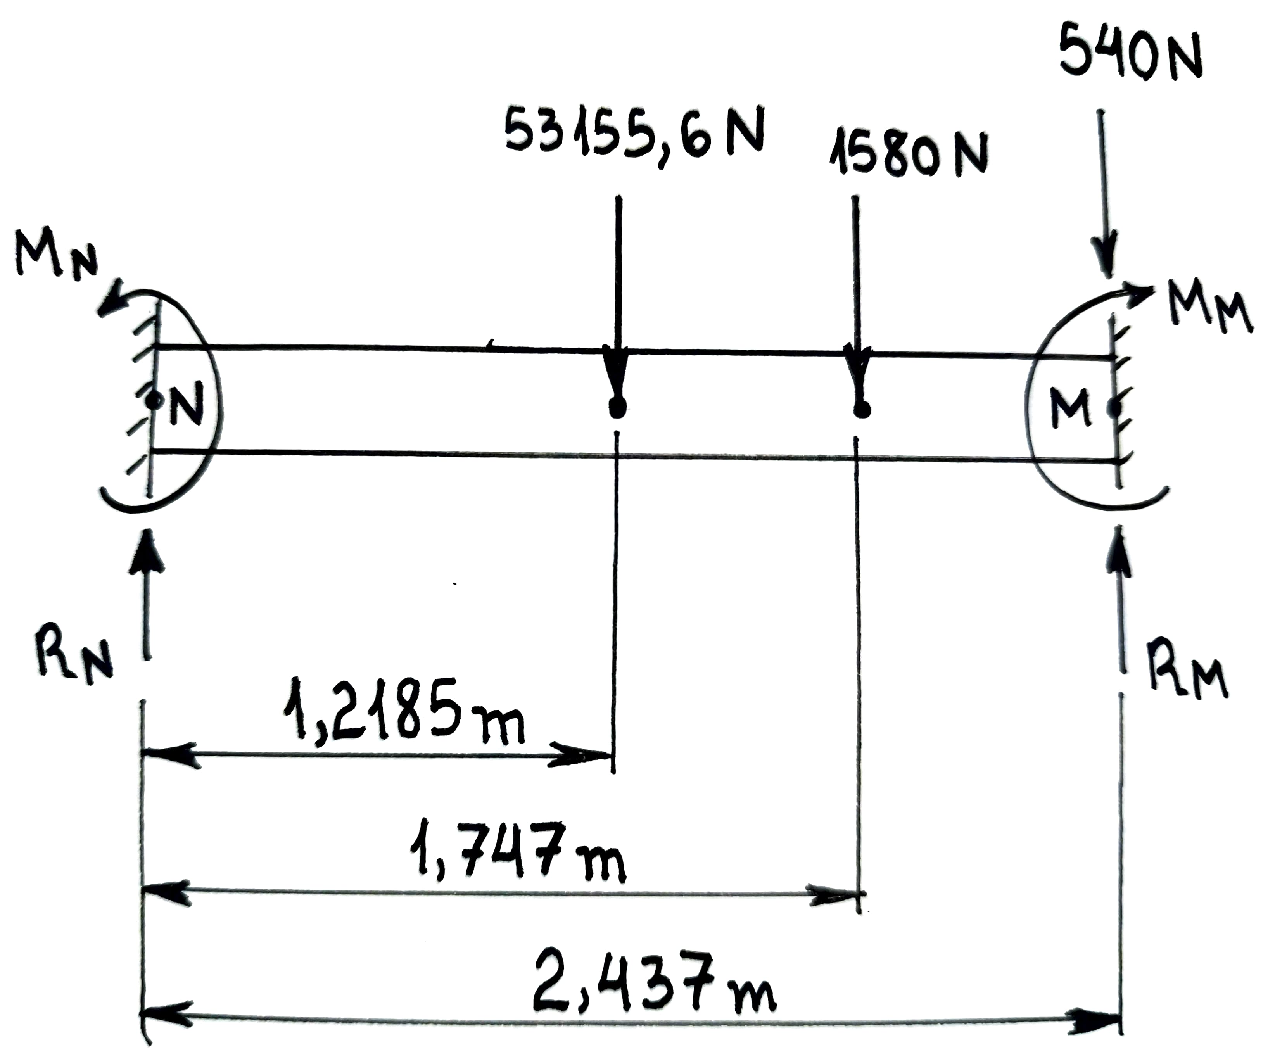
\includegraphics[width=0.8\textwidth]{content/sections/04_estrutura/sections/01_pre_dimensionamento_da_viga_vl2/figures/dcl_vl2.pdf}
  \caption{DCL da viga VL2 (Autor)}
  \label{fig:dcl_vl2}
\end{figure}

Para calcular as reações de apoio, é necessário aplicar as equações de equilíbrio estático:

\begin{flalign*}
   & \sum F_y = 0                                           &  & \\
   & R_N + R_M - \num{53155.6} - \num{1580} - \num{540} = 0 &  &
\end{flalign*}

\begin{equation}
  R_N + R_M - \num{55275.6} = 0
  \label{eq:sum_fy_vl2}
\end{equation}

\vspace{1em}

Os momentos atuantes no ponto N são:

\begin{equation*}
  \num{2.437} \cdot R_M
\end{equation*}

\begin{equation*}
  -\num{1.2185} \cdot \num{53155.6} = \SI{-64770.1}{\newton\meter}
\end{equation*}

\begin{equation*}
  -\num{1.747} \cdot \num{1580} = \SI{-2760.26}{\newton\meter}
\end{equation*}

\begin{equation*}
  -\num{2.437} \cdot \num{540} = \SI{-1315.98}{\newton\meter}
\end{equation*}

\begin{flalign*}
   & \sum M_N = 0                                                                    &  & \\
   & M_N - M_M - \num{64770.1} - \num{2760.26} - \num{1315.98} + \num{2.437} R_M = 0 &  &
\end{flalign*}

\begin{equation}
  M_N - M_M + \num{2.437} R_M - \num{68846.34} = 0
  \label{eq:sum_mn_vl2}
\end{equation}

Como o sistema é hiperestático, é necessário utilizar o método das funções de singularidade para obter a equação do momento fletor e integrar duas vezes para obter as equações da declividade e da linha elástica, assim se obtém as equações necessárias para concluir o cálculo das reações de apoio.

\begin{align*}
  M(x) & = R_N \left<x\right>^1 - M_N \left<x\right>^0 -\num{53155.6} \left<x - \num{1.2185}\right>^1 - \num{1580} \left<x - \num{1.747}\right>^1 \rightarrow         \\
       & \quad - \num{540} \left<x - \num{2.437}\right>^1 + R_M \left<x - \num{2.437}\right>^0 + M_M \left<x - \num{2.437}\right>^0 \left[ \si{\newton\meter} \right]
\end{align*}
